%!TEX root = ../vkr.tex

\section{Предварительная подготовка}
\subsection {Основные определения и обозначения}
\Def {Нейронная сеть $ \mathnormal{f}_{\theta}( \mathnormal{x})$ глубины $r$ это функция, параметризированная по $\theta$, которая берёт входы из входного пространства $\mathcal X$ и возвращает значения из выходного пространства $\mathcal Y$. Функция $ \mathnormal{f}$ составляется как последовательность функций, чередующихся между линейными слоями $ \mathnormal{f}_{ j}$ и нелинейной функцией $\sigma$:
 $$ \mathnormal{f} =  \mathnormal{f}_{r+1} \circ \sigma \circ \dots \circ \sigma \circ  \mathnormal{f}_{2} \circ \sigma \circ  \mathnormal{f}_{1}$$.}

Мы рассматриваем глубокие нейронные сети (DNN) на вещественных числах. Тогда, $\mathcal{X} = \mathbb{R}^{d_{0}}$ и $\mathcal{Y} = \mathbb{R}^{d_{r+1}}$, где $d_{0}$ и $d_{r+1}$ положительные целые. Также, в работе рассматриваются только нейронные сети с функцией активации ReLU $\sigma \colon \mathnormal{x} \mapsto max \left(\mathnormal{x}, ~0\right).$

\Def {  $i$-ый слой нейронной сети $ \mathnormal{f}_{i}$ задаётся как аффинное преобразование $$ \mathnormal{f}_{i}( \mathnormal{x}) = A^{\left (i \right )} \mathnormal{x} + b^{\left (i \right )}.$$ Веса $A^{\left (i \right )} \in {\mathbb {R}}^{d_{i} \times d_{i-1}}$ это ${d_{i} \times d_{i-1}}$-матрица; смещение $b^{\left ( i \right )} \in {\mathbb {R}}^{d_{i}}$ это $d_{i}$-мерный вектор.}

\Def {Нейрон $-$ это функция, определяемая соответствующей матрицей весов и функцией активации. В частности, $j$-ый нейрон слоя $i$ $-$ это функция $\eta$, заданная следующим образом 
$$\eta \left( \mathnormal{x}\right) = \sigma \left( A_{j}^{\left ( i \right )} \mathnormal{x} + b_{j}^{\left ( i \right )} \right).$$
Всего имеется $N=\sum_{j=1}^{r} d_{i}$ нейронов.}

\Def {Пусть $\mathnormal{l} = d_{i-1}$ и $A_{j}^{\left ( i \right )}$ описывается как $\left( a_{1}, a_{2}, \dots, a_{\mathnormal{l}}\right)$. Сигнатура $j$-ого нейрона слоя $i$ это кортеж 
\begin{equation}
	\label{eq1} \left( \frac{a_{1}}{a_{1}} = 1, \frac {a_{2}}{a_{1}}, \dots, \frac {a_{\mathnormal{l}}}{a_{1}} \right).
\end{equation}
}

\Def {Пусть $\mathcal{V} \left ( \eta {;}~  \mathnormal{x} \right )$ обозначает вход нейрона $\eta$ $\left ( \text{до применения } \sigma \right)$ при $\mathnormal{x} \in \mathcal{X}$. Нейрон $\eta$ является критическим, когда $\mathcal{V} \left ( \eta {;}  \mathnormal{x} \right ) = $ 0. Критической точкой $\eta$, назовём входной сигнал $\mathnormal{x}$, обозначаемый $\mathnormal{x} \in \mathcal{W}(\eta)$. Если $\mathcal{V} \left ( \eta {;}  \mathnormal{x} \right ) > $ 0 тогда нейрон активен, иначе $-$ неактивен. Состояние $\eta$ на входе $\mathnormal{x}$ (активное, неактивное или критическое) обозначается $\mathcal{S} \left(\eta {;}~ \mathnormal{x} \right)$.
}

\Def {Пусть $\mathnormal{x} \in \mathcal{X}$. Линейной окрестностью $\mathnormal{x}$ назовём множество
$$ \{ \mathnormal{u} \in \mathcal{X} \mid \mathcal{S} \left ( \eta {;}~ \mathnormal{x} \right ) = \mathcal{S} \left ( \eta {;}~ \mathnormal{u} \right ) \text{для всех нейронов } \eta \text{ в сети} \}.$$ } 

\Def {Архитектура нейронной сети описывается структурой $\mathnormal{f} {:}$ $\left(a\right)$ числом слоёв и $\left(b\right)$ размерностью каждого слоя $\{d_{i}\}_{i=0}^{k+1}$.}

Пусть $\mathnormal{F}_{i}$ обозначает функцию, которая вычисляет первые i слоёв DNN после функций ReLU, т.е. $\mathnormal{F}_{i} = \sigma \circ  \mathnormal{f}_{i} \circ \sigma \circ \dots \circ \sigma \circ  \mathnormal{f}_{1}$. По определению, все нейроны остаются в одном и том же состоянии при вычислении DNN с входами из линейной окрестности для $\mathnormal{x} \in \mathcal{X}$. Для каждой такой точки $\mathnormal{x}'$ имеем
\begin{align*}
\mathnormal{F}_{i} \left( \mathnormal{x}' \right)  &= I^{\left( i \right)} \left(A^{\left( i \right)} \dots \left( I^{\left( 2 \right)} \left( A^{\left( 2 \right)} \left ( I ^{\left( 1 \right)} \left (A^{\left( 1 \right)} \mathnormal{x}' + \mathnormal{b}^{\left( 1 \right)} \right) \right) + \mathnormal{b}^{\left( 2 \right)} \right) \right.  \dots + \mathnormal{b}^{\left( i \right)}\right)\\
&= I^{\left( i \right)} A^{\left( i \right)} \dots I^{\left( 2 \right)} A^{\left( 2 \right)} I^{\left( 1 \right)} A^{\left( 1 \right)} \mathnormal{x}' + \beta\\
&=\mathit{\Gamma} \mathnormal{x}' + \mathit{\beta},
\end{align*}
где $I^{\left(j \right)}$ это $0 - 1$ диагональная матрица с 0 на $k$-ом элементе диагонали, когда $k$-ый нейрон слоя $j$ неактивен и 1 на $k$-ом элементе диагонали, когда нейрон активен. То есть, в линейной окрестности входного сигнала $\mathnormal{x}$ мы можем "свернуть" действие различных смежных слоёв в аффинной преобразование. Если мы изменяем вход на $\mathit{\Delta}$, то можем наблюдать соответствующие изменения в значении нейронов:
$$\mathnormal{F}_{i} \left( \mathnormal{x} + \mathit{\Delta} \right) - \mathnormal{F}_{i} \left( \mathnormal{x} \right) = \mathit{\Gamma} \left(\mathnormal{x} + \mathit{\Delta} \right) + \beta - \left(\mathit{\Gamma} \left(\mathnormal{x}\right) + \beta\right) = \mathit{\Gamma}\mathit{\Delta}.$$
Это $\mathit{\Delta}$ должно быть таким, чтобы $\mathnormal{x} + \mathit{\Delta}$ находилось в линейной окрестности $\mathnormal{x}$.

Предположим, что нам полностью известны первые $i-1$ слоев, и в данный момент мы восстанавливаем слой $i$. Пусть $\mathnormal{F}_{i-1}$ и $\mathnormal{G}_{i+1}$ представляют собой, соответственно, полностью восстанновленную и невостановленную части DNN, т.е
$$ \mathnormal{f} = \underbrace{\mathnormal{f}_{k+1} \circ \sigma \circ \dots \circ \sigma \circ  \mathnormal{f}_{i+1}}_{\mathnormal{G}_{i+1}} \circ \sigma \circ \mathnormal{f}_{i} \circ \underbrace{\mathnormal{f}_{i-1} \circ \sigma \circ \dots \circ \sigma \circ  \mathnormal{f}_{1}}_{\mathnormal{F}_{i-1}}.$$


\begin{figure}[h]
\center{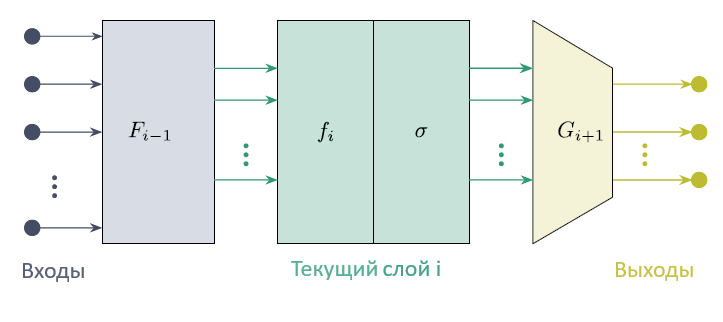
\includegraphics[width=1\linewidth]{i-dnn}}
\caption{Представление DNN в соответствии с восстановленной частью $\mathnormal{F}_{i-1}$, текущим целевым слоем $i$ и неизвестной частью $\mathnormal{G}_{i+1}$.}
\label{ris:i-dnn}
\end{figure}

Тогда, нейронную сеть можно изобразить так, как показано на рисунке $\ref{ris:i-dnns}$. Более того, если мы ограничим входы $\mathnormal{x}'$ линейной окрестностью $\mathnormal{x}$, мы можем свернуть $\mathnormal{F}_{i-1}$ и $\mathnormal{G}_{i+1}$ как
\begin{align*}
\mathnormal{F}_{i-1} \left (\mathnormal{x}' \right)& = \mathnormal{F}_{\mathnormal{x}}^{\left(i-1\right)} \mathnormal{x}' + \mathnormal{b}_{\mathnormal{x}}^{\left(i-1\right)}     & \text{и}         &  &\mathnormal{G}_{i+1} \left (\mathnormal{x}' \right) = \mathnormal{G}_{\mathnormal{x}}^{\left(i+1\right)} \mathnormal{x}' + \mathnormal{b}_{\mathnormal{x}}^{\left(i+1\right)},
\end{align*}
соответственно. Подстрочный индекс $\mathnormal{x}$ в свёрнутых матрицах и векторах смещения означает, что они определнены в линейной окрестности $\mathnormal{x}$.

\Def {$j$-ая строка $\mathnormal{G}_{\mathnormal{x}}^{\left(i+1\right)}$ есть выходные коэффициенты $j$-ого выхода DNN.}

\subsection {Постановка задачи и допущения}

\Def {Атака с извлечением параметров модели получает оракульный доступ к параметризированной функции $ \mathnormal{f}_{\theta}$ (в нашем случае нейронная сеть глубины $k$) и архитектуре $ \mathnormal{f}$, и возвращает набор параметров $\widehat{\theta}$ с целью, чтобы $ \mathnormal{f}_{\theta}( \mathnormal{x})$ была как можно более похожа на  $ \mathnormal{f}_{\hat{\theta}}( \mathnormal{x})$. }
Восстановление параметров слой за слоем происходит в два этапа. На первом этапе находятся кратные параметры, в частности, сигнатуры нейронов $\ref{eq1}$. Поскольку сигнатура состоит из соотношений пар весов, одновременное отрицание всех этих весов сохранит сигнатуру, но нелинейно изменит выходы ReLU данного нейрона. Следовательно, прежде чем отделить слой нейронов, необходимо определить знак весов этого нейрона. На втором этапе эти знаки восстанавливаются для всех нейронов в текущем слое.

Сделаем некторые предположения относительно оракула и возможностей атакующего:
\begin{itemize}
\item
	 $\textbf{Знание архитектуры}$. Нам требуется знать архитектуру нейронной сети.
\item
	 $\textbf{Полнодоменные входы}$. Мы подаём на вход произвольные сигналы из $\mathcal X = \mathbb{R}^{d_0}$.
\item
	 $\textbf{Полные выходы}$. Мы получаем выходные данные непосредственно от модели $ \mathnormal{f}$ без дополнительной оработки.
\item
	 $\textbf{Точные вычисления}$.Для задания и оценки $ \mathnormal{f}$ используется $64$-разрядная арифметика с плавающей запятой.
\item
	 $\textbf{Скалярные выходы}$. Без потери общности считаем, что размерность выхода равнна $1$, т.е. $\mathcal Y = \mathbb {R}$.
\item
	 $\textbf{Полносвязная сеть и активация ReLU}$. Сеть я вляется полностью соединённой, и все функции активации $\left ( \sigma \right )$ являются функциями ReLU.
\item
	 $\textbf{Доступность и уникальность подписи}$. Мы имеем доступ к сигнатуре каждого нейрона. Кроме того, мы предполагаем, что нет двух одинаковых сигнатур.

\end{itemize}